\chapter{Uvod}

Ovaj završni projekt se izvodi u sklopu projekta FERSAT, koji se od 2018. godine provodi na Fakultetu elektrotehnike i računarstva Sveučilišta u Zagrebu \cite{fersat_stranica_projekta}. Cilj projekta je izrada, lansiranje i korištenje nanosatelita u CubeSat formatu, dimenzija 10 cm x 10 cm x 10 cm, volumena jedne litre i težine ne veće od 4/3 kg. Navedene dimenzije satelita odgovaraju formatu CubeSat 1U. Planirana visina orbite satelita je između 500 i 600 km, a očekivano trajanje misije je 3 godine. 
 
Korisni teret satelita (engl. \textit{payload}) se sastoji od tri podsustava:

\begin{itemize}
	\item kamera za snimanje površine Zemlje i zemaljskog horizonta,
	\item detektori svjetla u vidljivom i ultraljubičastom dijelu spektra za mjerenje svjetlosnog onečišćenja i debljine stupca ozona,
	\item komunikacijski sustav u radijskom X-pojasu (10.45 GHz) za prijenos podataka na Zemlju.
\end{itemize}

Kako bi se moglo upravljati radom korisnog tereta, na satelit će biti ugrađeno PDH (engl. \textit{Payload Data Handler}) računalo, čija će zadaća biti prikupljanje podataka s kamere i senzorskog podsustava, pohranjivanje prikupljenih podataka u trajnu memoriju (engl. \textit{non-volatile memory}), te slanje podataka na Zemlju pomoću komunikacijskog sustava. Izabrani mikrokontroler za ulogu PDH računala je STM32L471VGT6 proizvođača ST Microelectronics.
U okviru ovog završnog projekta razvijen je dio programske potpore za računalo zaduženo za upravljanje korisnim teretom satelita.

Ostalim podsustavima, koji nisu direktno vezani uz koristan teret, upravlja CDH (engl. \textit{Command and Data Handler}) računalo. CDH računalo može upravljati položajem i orijentacijom satelita, slanjem telemetrijskih podataka na Zemlju, a također upravlja i napajanjem korisnog tereta i šalje naredbe PDH računalu preko CAN (engl. \textit{Controller Area Network}) sučelja. U trenutku pisanja ove dokumentacije, konkretno CDH računalo još nije odabrano.
    
Slika \ref{fig:fersat_blok_ks} prikazuje blok dijagram cijelog sustava. U okviru ovog projekta razvijena je programska potpora PDH računala za upravljanje kamerom i \textit{flash} memorijom.

\begin{figure}[H]
	\centering
	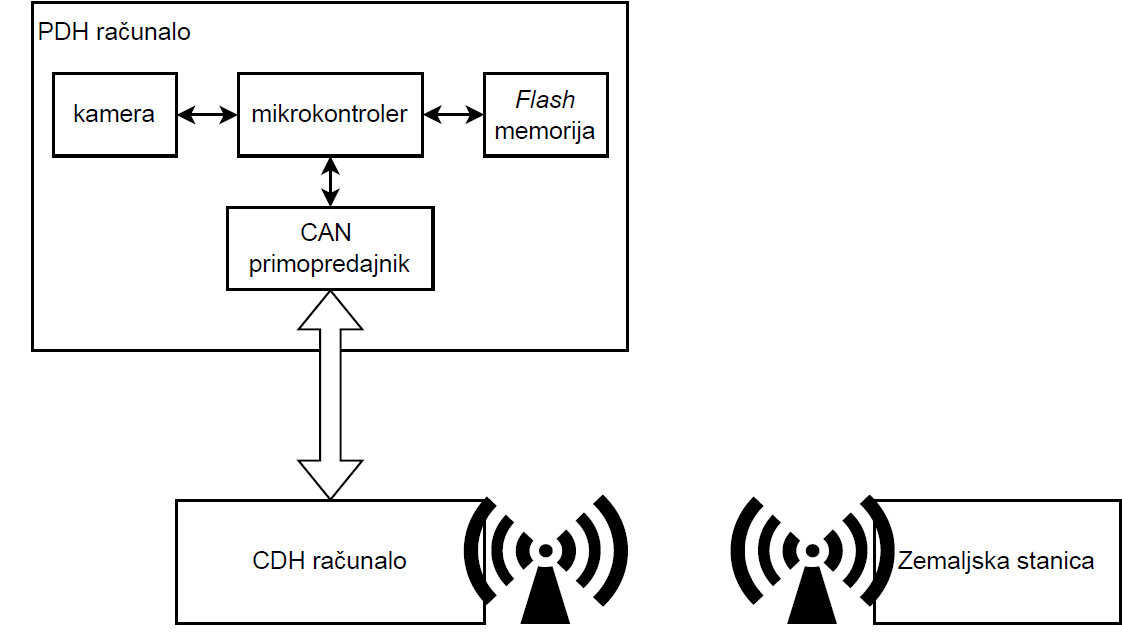
\includegraphics[width=\textwidth]{fersat_blok_dijagram_ks.png}
	\caption{Blok dijagram FERSAT-a i komunikacija sa zemaljskom postajom \cite{diplomski_goran_petrak}}
	\label{fig:fersat_blok_ks}
\end{figure}

Sustav za upravljanje kamerom se sastoji od Arducam Mini 5MP Plus kamere. Upravljanje kamerom se sastoji od konfiguracije kamere i samog korištenja kamere, odnosno slikanja i spremanja slike. Konfiguracija kamere je nužna kako bi se ispravno podesili parametri trajanja ekspozicije, pojačanje i formata u kojem se slika želi spremiti.

S obzirom na to da je u ovom završnom projektu naglasak bio na prilagođavanju postojeće programske podrške, u ovom radu će biti raspravljeni izazovi i izmjene do kojih je došlo tijekom prilagođavanja programske podrške. Poglavlje 2 sadrži kratak pregled arhitekture PDH sustava. U poglavlju 3 dan je detaljan opis I\textsuperscript{2}C (engl. \textit{Inter-Integrated Circuit}) i SPI (engl. \textit{Serial Peripheral Interface}) sučelja koja se koriste za komunikaciju s kamerom i \textit{flash} memorijom. Posebno su istaknute razlike između starog i novog periferijskog sklopovlja koje su bile ključne za prilagođavanje programske podrške. U poglavlju 3 je također objašnjen CAN protokol i dan je detaljan uvid u način rada CAN periferijskog sklopovlja na mikrokontroleru. Detaljan pregled razvijene programske podrške dan je u poglavlju 4, gdje je opisana integracija programske podrške za kameru i \textit{flash} memorija u FreeRTOS operacijski sustav za rad u stvarnom vremenu i način korištenja CAN periferije. U poglavlju 5 izloženi su rezultati projekta i način korištenja sustava.